\chapter{视觉问答任务及基础架构}
虽然视觉问答任务是从2014年才被提出的新兴人工智能领域,但是由于其跨学科的特性以及图像处理和自然语言处理领域的快速发展,目前视觉问答模型迭代速度也非常快,大量的数据集、模型被提出。本章将介绍视觉问答研究中重要的基础知识和模型的基础架构。

\section{视觉问答任务}
视觉问答是向智能系统给出图片和问题,系统返回答案的任务。由于图像内容的复杂性和问题的开放性,视觉问答的研究难度较大,正因如此,其相较于其他子任务更接近通用人工智能。本节我们将详细分析其问题类型,并介绍目前主要的数据集。
\subsection{问题类型划分}
由于视觉问答任务的最终目的是面向真实的人类交互场景,因此VQA模型需要解决开放性问题的挑战,问题类型的研究是构建模型前的关键步骤之一。

按照问题的形式划分,视觉问答的问题可以分为二值否问题\citing{krishna2017visual,zhu2016visual7w,andreas2015deep}、多选问题\citing{antol2015vqa,zhu2016visual7w}、开放性问题\citing{antol2015vqa}。按照问题的内容划分,问题分为识别类和推理类。识别类问题包括物体识别、物体检测、属性分类、计数问题、空间关系判定,此类任务在以往的计算机视觉的研究中已经达到了较高的识别准确率,在某些物体识别和物体检测任务上已经能迫近甚至超越人类水平。推理类问题包括场景识别、常识推理和知识库推理等,这类问题形式多变、层次复杂、需要外源知识、甚至需要多步推理,例如:“图片中有什么东西在伞下?”——需要能准确识别物体的空间位置关系、“图片中的交通路口是否可以通行?”——需要基于常识的推理、“图片中的汽车属于什么品牌?”——需要基于外部专业知识库提供隐藏信息。

除了以上提到的两种问题分类,本文提出了一种全新问题分类标准——按照答案与问题和图像的相关性划分。我们认为:对于不同的视觉问答问题,其答案-图像相关度、答案-文本相关度存在差异,即有的答案更依赖于准确的图像分析,而有的答案却对图像不敏感。而这种与输入信息的相关性差异能帮助我们更好的理解模型决策的内部机制。我们提出以Q、q、I、i定性的表示“答案-问题强相关”、“答案-问题弱相关”、“答案-图像强相关”、“答案-图像弱相关”,从而组合得出四种问题类型QI、Qi、qI、qi,如表\ref{ques_type}所示。
\begin{table}[H]
% \resizebox{0.8\textwidth}{!}{}
\centering
\caption{根据答案和源信息的相关性划分出四类任务}
\begin{tabular*}{0.9\textwidth}{@{\extracolsep{\fill}}lccc}
\toprule
& \textbf{答案-问题相关性} & \textbf{答案-图像相关性} & \textbf{问题类型} \\
\midrule
\multirow{4}{*}{\textbf{相关性}} &  强& 强&  QI\\
&  强& 弱&  Qi\\
&  弱& 强&  qI\\
&  弱& 弱&  qi\\
\bottomrule
\end{tabular*}
\label{ques_type}
\end{table}

QI类型的问题需要同时结合图像特征和文本特征,这是一种最典型的视觉问答类型。Qi类型的问题答案可以直接根据问题文本得出,这类图像无关的问题可以退化为文本问答任务。qI类型的答案可以直接从图像中得出,这类问题退化为图像识别任务。例如,对于图\ref{DogExample},问题1:“图片中的狗是什么颜色?”,模型可以通过直接识别出图像中狗的色彩属性得出正确答案,那么问题1就是qI类型。对于同样的图片,问题2:“图片上的狗是不是属于动物?”是图像无关的Qi类型。
\begin{figure}[H]
	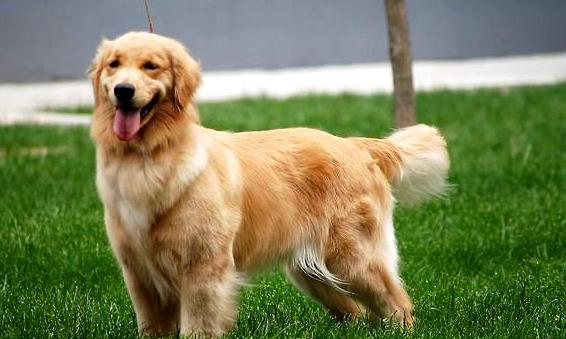
\includegraphics[width=0.8\textwidth]{DogExample.jpg}
	\caption{视觉问答示例图}
	\label{DogExample}
\end{figure}

qi类型的问题答案与问题文本和图像的相关性都比较弱,这类问题包含两类类型,一类为错误或者偏僻的问题,例如偏僻单词的问题、低频的语法结构;另一类为涉及常识和外源知识的问题,回答这类问题需要额外的知识,甚至还需要多步的推理,例如,对于图\ref{DogExample},问题3:“图片中的动物是什么颜色?”,模型除了需要正确识别图片中的狗和颜色属性,还需要知道“狗属于动物”的常识,才能在“狗的颜色”——黄色和“草地的颜色”——绿色之间做出正确的预测。目前,对于错误或者偏僻的qi问题研究较少。

\subsection{视觉问答数据集}
视觉问答任务是在经历了计算机视觉和自然语言处理任务成功之后,新兴出现的人工智能任务——要求系统能同时理解多模信息,并完成信息整合与推理。自从2014年以来,多个高质量的视觉问答数据集被提出:DAQUAR\citing{malinowski2014multi}、COCO-QA\citing{ren2015exploring}、VQA\citing{antol2015vqa}、VQA 2.0\citing{goyal2017making}、CLEVR\citing{johnson2017clevr}、KB-VQA\citing{wang2015explicit}、FVQA\citing{wang2017fvqa}。

以上的数据集有不同的图像来源,各自的问题对的数量也不同,但是其中最重要的区别在于问题回答是否需要额外知识,例如常识和专业知识。我们将不需要额外知识的数据集称为“基于视觉的数据集”——问题的答案往往来源于图像信息的准确提取,而需要额外知识的数据集称为“基于知识的数据集”——图像信息仅仅作为推理的一环,答案依赖于图像和问题以外的知识。根据以上的划分标准,以上提到的数据集的统计信息如表\ref{dataset_compar}。正如表格所示,KB-VQA和FVQA属于“基于知识的数据集”,其他均属于“基于视觉的数据集”。
\begin{table}[H]
% \resizebox{0.8\textwidth}{!}{}
\centering
\caption{视觉问答数据集的对比,其中KB-VQA和FVQA属于“基于知识的数据集”,其他均属于“基于视觉的数据集”。}
\begin{tabular*}{0.9\textwidth}{lrrcc}
\toprule
\textbf{Dataset} & \textbf{\#images} & \textbf{\#QA pairs} & \textbf{Image source} & \textbf{Knowledge based}\\
\midrule
DAQUAR\citing{malinowski2014multi}&  1,449& 12,468&  NYU-Depth& \\
COCO-QA\citing{ren2015exploring}&  69,172& 117,684&  COCO& \\
VQA\citing{antol2015vqa}&  204,721& 614,163&  COCO& \\
VQA 2.0\citing{goyal2017making}&  204,721& 1,105,904&  COCO& \\
CLEVR\citing{johnson2017clevr}&  100,000& 999,968&  Synthetic images& \\
\midrule
KB-VQA\citing{wang2015explicit}&  700& 2402&  COCO+ImgNet& $\surd$\\
FVQA\citing{wang2017fvqa}&  1,906& 4,608&  COCO& $\surd$\\
\bottomrule
\end{tabular*}
\label{dataset_compar}
\end{table}

\subsubsection{基于视觉的数据集}
\textbf{DAQUAR}\qquad
DAQUAR从NYU-Depth V2中带有语义分割标注的图片基础上扩展而来\citing{malinowski2014multi}。数据集包含1449张图片,图片多为室内场景,这大大地限制了数据集的场景丰富性,是该数据集的一大劣势。数据集由训练集和测试集两部分组成,训练集中包含6794对“问题-答案”,测试集中包含5674对“问题-答案”,“问题-答案”对由算法生成或是人类志愿者提供,算法生成的“问题-答案”对根据给定的模板生成。
% \begin{figure}[H]
% 	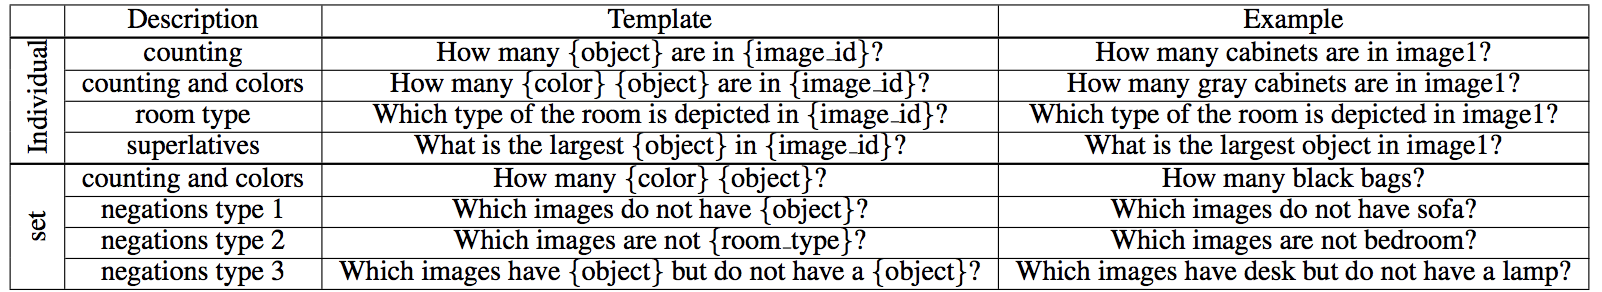
\includegraphics[width=0.8\textwidth]{DAQUAR.png}
% 	\caption{DAQUAR问题模板}
% 	\label{DAQUAR}
% \end{figure}

% DAQUAR数据集较小并且问题的类型只有三种:物体识别、色彩识别、计数,并且答案类型多以单词为主,因训练和测试系统复杂问题的推理能力较弱,偏于传统的物体识别任务。

\textbf{COCO-QA}\qquad
COCO-QA包含来自MS COCO的123287张真实场景图片,问题-答案对则是运用算法从MS COCO数据集的图像标注中生成的,为了方便生成算法的运用,将问题划分在物体识别、色彩识别、计数、地点查询四种类型。DAQUAR数据集在实际测试过程中,被发现仅仅通过简单的猜测答案的方式都能获得较高的正确率,这使得高准确率出现了极大的偏差,不能公正的测试系统的“推理”能力。为了克服该缺点,COCO-QA去除了出现频数极低和极高的一些答案,使得常见答案出现的评率从24.98\%下降到7.30\%。COCO-QA的训练集包含78736对“问题-答案”,测试集包含38948对“问题-答案”。
% 在四个类别中的分布如图\ref{coco-vqa}。
% \begin{figure}[H]
% 	\centering
% 	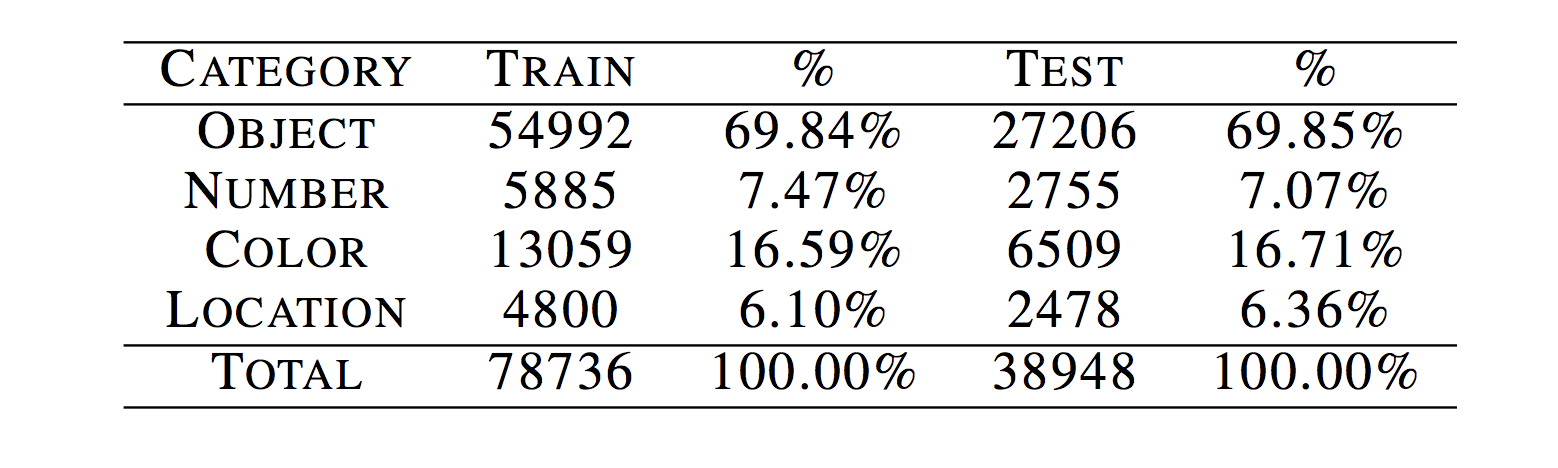
\includegraphics[width=0.8\textwidth]{coco-vqa.png}
% 	\caption{coco-vqa中“问题-答案”对的分布情况}
% 	\label{coco-vqa}
% \end{figure}

\textbf{VQA}\qquad
VQA数据集是视觉问答领域发展的一个重要拐点,在此之前的数据集的问题类型被限制在一些模板之中,这使得数据集不能很好地测试出视觉问答系统在真实语境下的表现,例如,DAQUAR将答案仅仅限制在16种基本颜色和894种物体类别中\citing{malinowski2014multi}。VQA数据集中的问题和答案是无限制、开放式的,且全部由人类产生,同时图片的数量相较DAQUAR提高了两个数量级,到达254731张,极大的提高了数据集的容量。VQA数据集不仅包含从MS COCO\citing{lin2014microsoft}中提取的204721张真实场景的图片,还提供了50000张合成的抽象场景图,丰富了数据库场景的多样性,同时为高阶的场景推理和复杂空间推理提供了便利。
% \begin{figure}[H]
% 	\centering
% 	\subfigure[真实场景图像实例]{
% 		\label{vqa-real}
% 		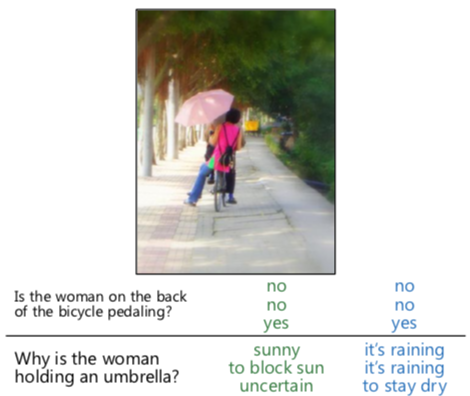
\includegraphics[width=0.4\textwidth]{VQA-real.png}}
% 	\subfigure[抽象场景图像实例]{
% 		\label{vqa-abs}
% 		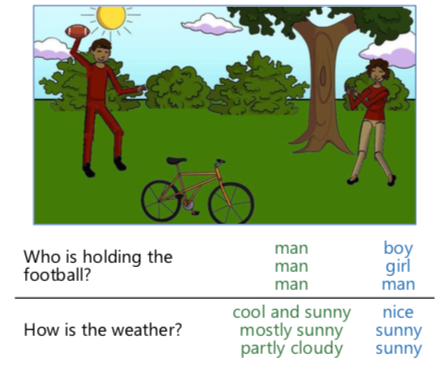
\includegraphics[width=0.4\textwidth]{VQA-abs.png}}
% 	\caption{VQA中的真实、抽象场景图像实例}
% 	\label{vqa-exmaple}
% \end{figure}

% 为了实现对复杂推理的训练和测试,VQA数据集在问题设置上采用了人工的方式,每张图片都有3个人类提出的问题。答案则分为开放式和多项选择两种形式,开放式答案由于答案并不唯一,因此难以确定标准答案,因此正确答案的评估方法也引入人工评估机制:对于同一个开放性问题由十个人分别作答,如果有三个及以上的被测者均提供了同一答案,该答案被视为正确答案。多项选择的答案则由四种类型、18个候选项组成(如图\ref{vqa-multi}):
% \begin{description}[labelindent=2em, leftmargin=6em, style=sameline]  
% \item [正确答案] 一个,从被测者回答中取最为常见的作为正确答案
% \item [混淆答案] 三个,不看图,仅根据问题作答的答案
% \item [常见答案] 十个,数据集中最出现频数最高的十个答案
% \item [随机答案] 四个,除去已经列出的选项,随机挑选四个答案
% \end{description}
% \begin{figure}[H]
% 	\centering
% 	\subfigure[真实场景图像的多选实例]{
% 		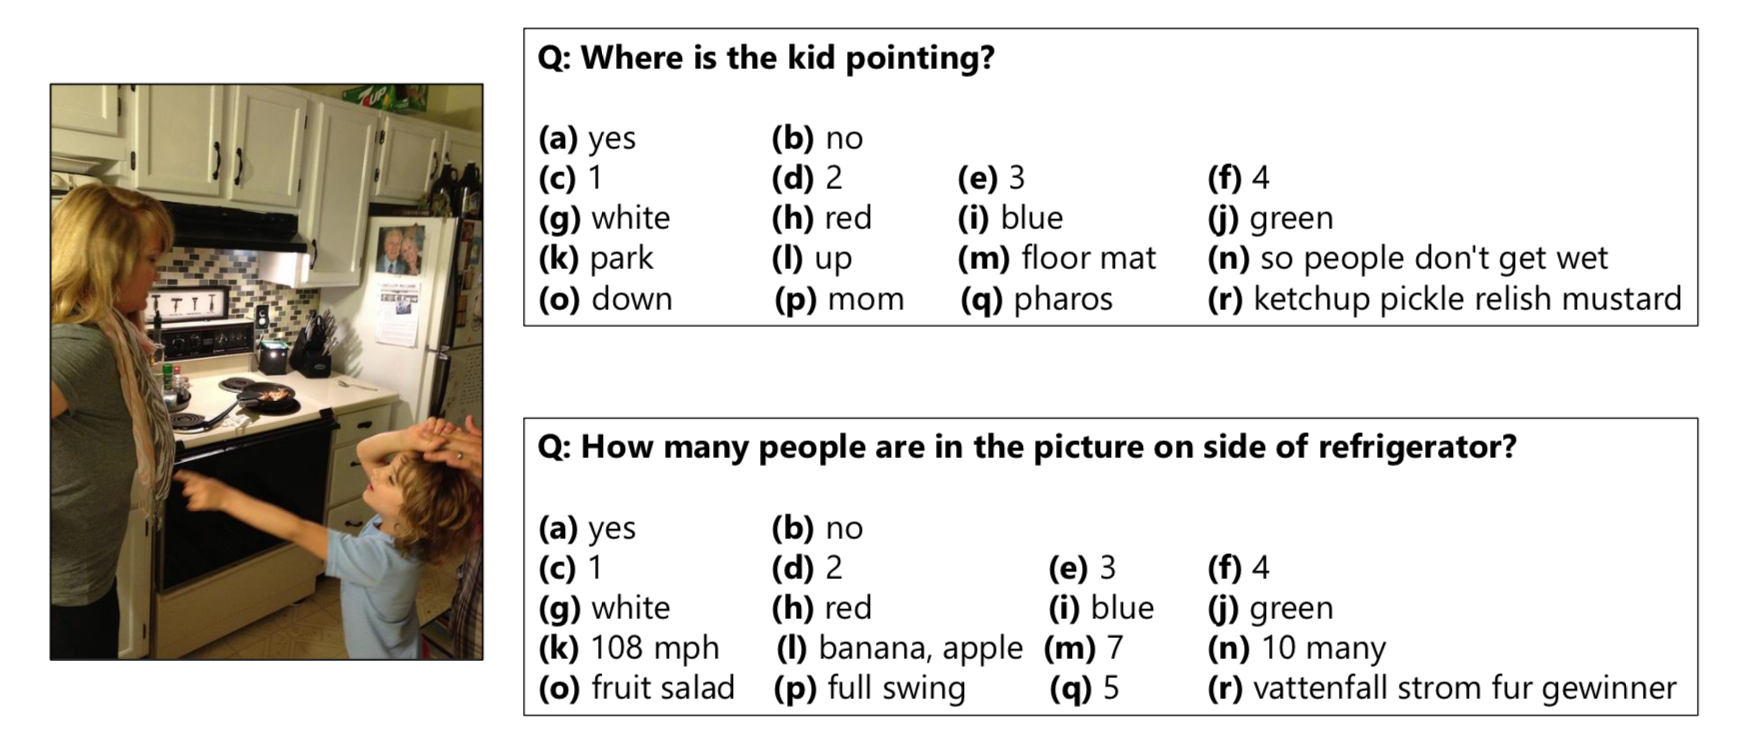
\includegraphics[width=0.8\textwidth]{vqa-multi.png}}
% 	\subfigure[抽象场景图像的多选实例]{
% 		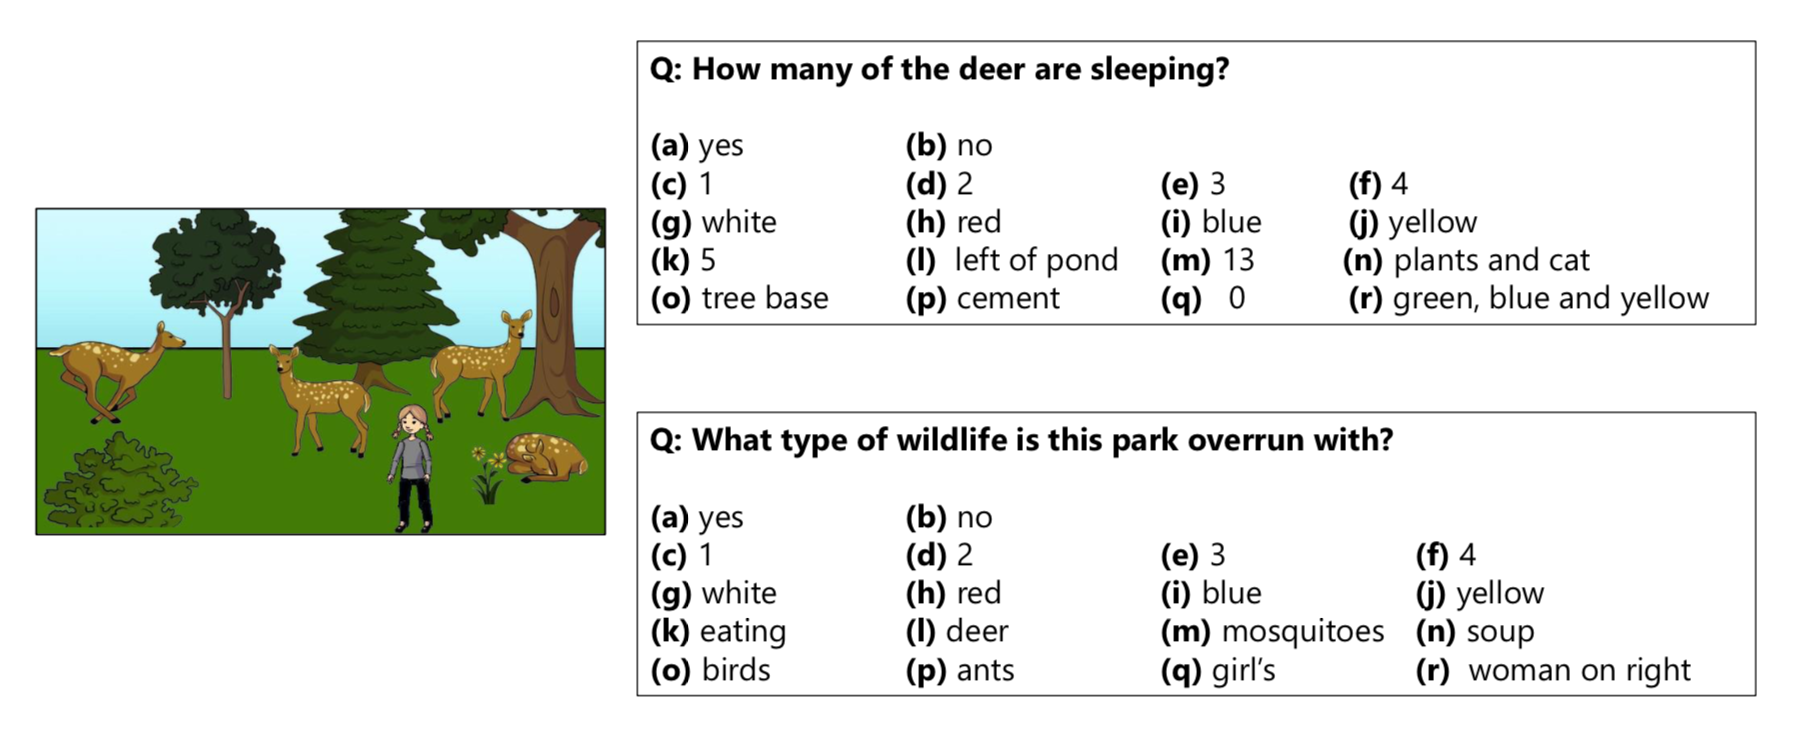
\includegraphics[width=0.8\textwidth]{vqa-multi2.png}}
% 	\caption{VQA中的真实和抽象场景图像的多项选择实例}
% 	\label{vqa-multi}
% \end{figure}


% VQA数据集由于其建立了开放性问题和多项选择问题的评测标准,成为众多算法的测试数据集,但VQA数据集存在语言偏见问题。具体表现为,即使是完全无视图像的算法也能在VQA数据集上得到49.6\%的准确率\citing{ren2015exploring},这意味在VQA数据集的测试环境下,系统对于视觉信息的需求程度远远小于语言信息,这种状况相较于人类对于图像问答任务中的真实体验而言,是严重不符的。例如,答案为”是或否“的问题占所有问题的38\%,并且大约59\%的二值问题答案都为”是“;询问”什么运动“的问题中有41\%的答案为”网球;询问数量的问题中有39\%的答案为“2”。
\textbf{VQA 2.0}\qquad
针对VQA数据集的语言偏见问题,VQA 2.0通过在原有的VQA数据集基础上补充新的“混淆数据”实现数据集对视觉信息的增强。“混淆数据”和原始数据一样由(图像I,问题Q,答案A)的形式组织,不同的是新补充的图像与原有图像相似,但回答同样的问题Q却得到不同的答案A。针对同样的问题,在不同图片背景下需要得到不同的答案,这要求系统不仅能理解自然语言问题,同样需要关注图片的语义差异,才能得到正确的答案,这种平衡的方法能够筛选掉弱化图像理解的算法,强化了图像理解在视觉问答任务的重要性。补充后的VQA 2.0包含110万对”图像-问题“、20万张关联1300百万个问题的真实场景图片,数据量几乎是VQA数据集的两倍,成为了开放性问题的新测试标准。
% \begin{figure}[H]
% 	\centering
% 	\subfigure[]{
% 		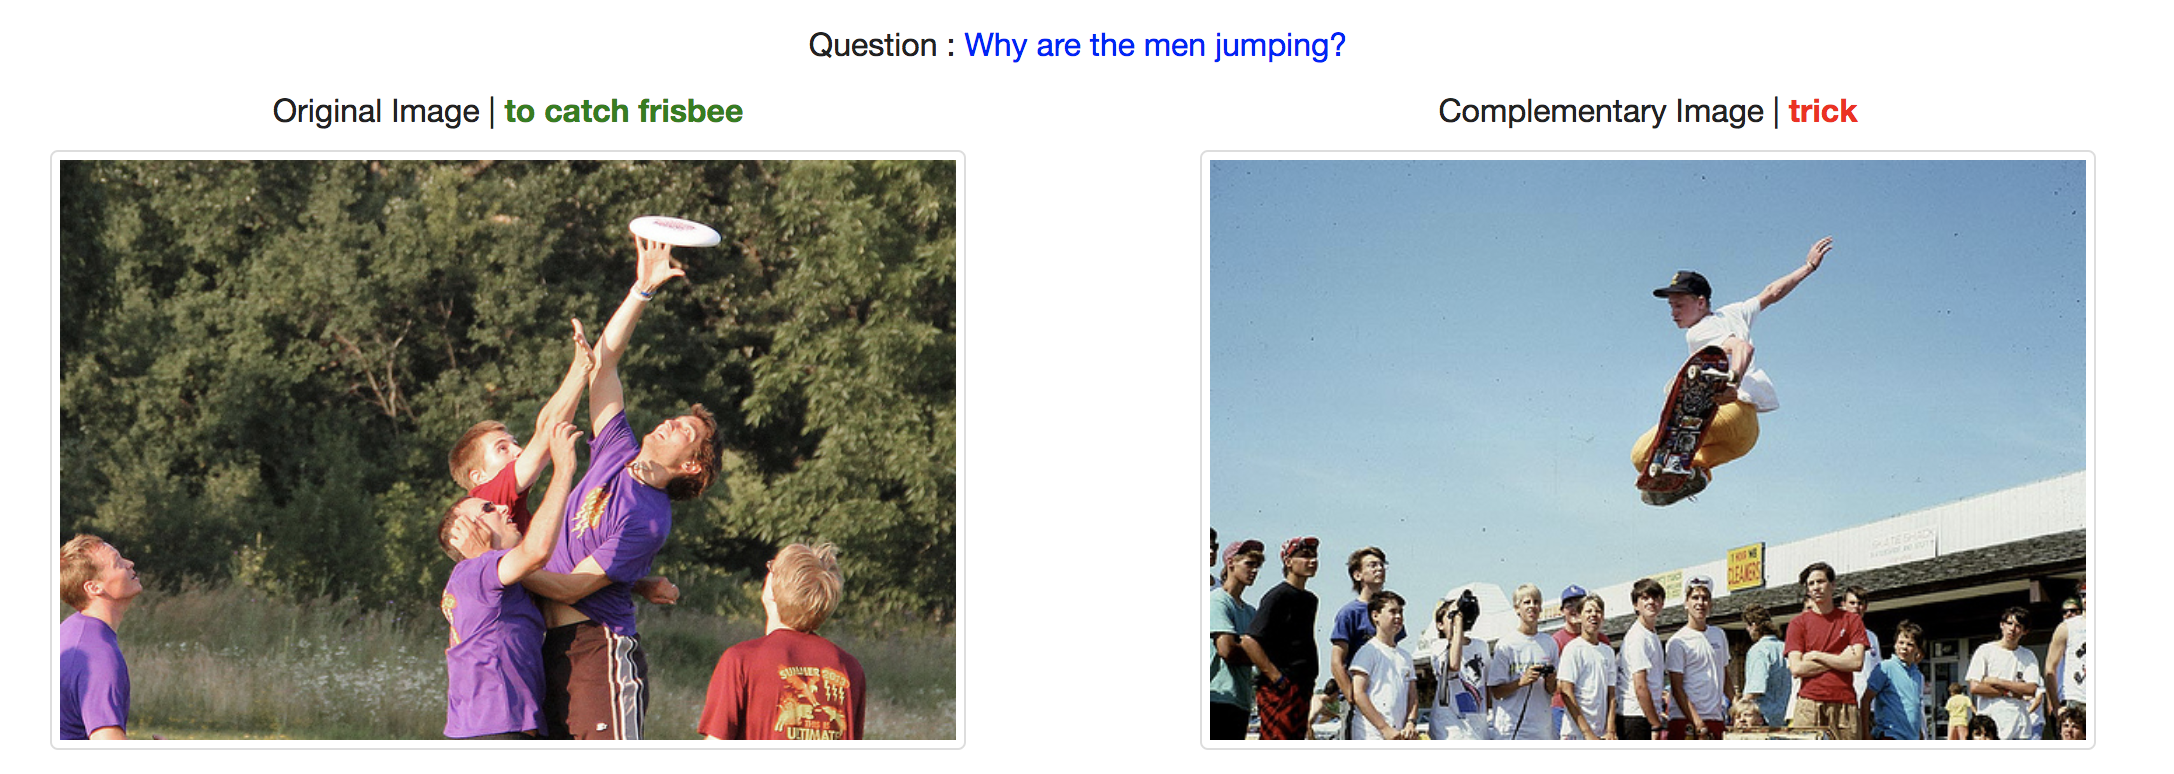
\includegraphics[width=0.8\textwidth]{vqa2-1.png}}
% 	\subfigure[]{
% 		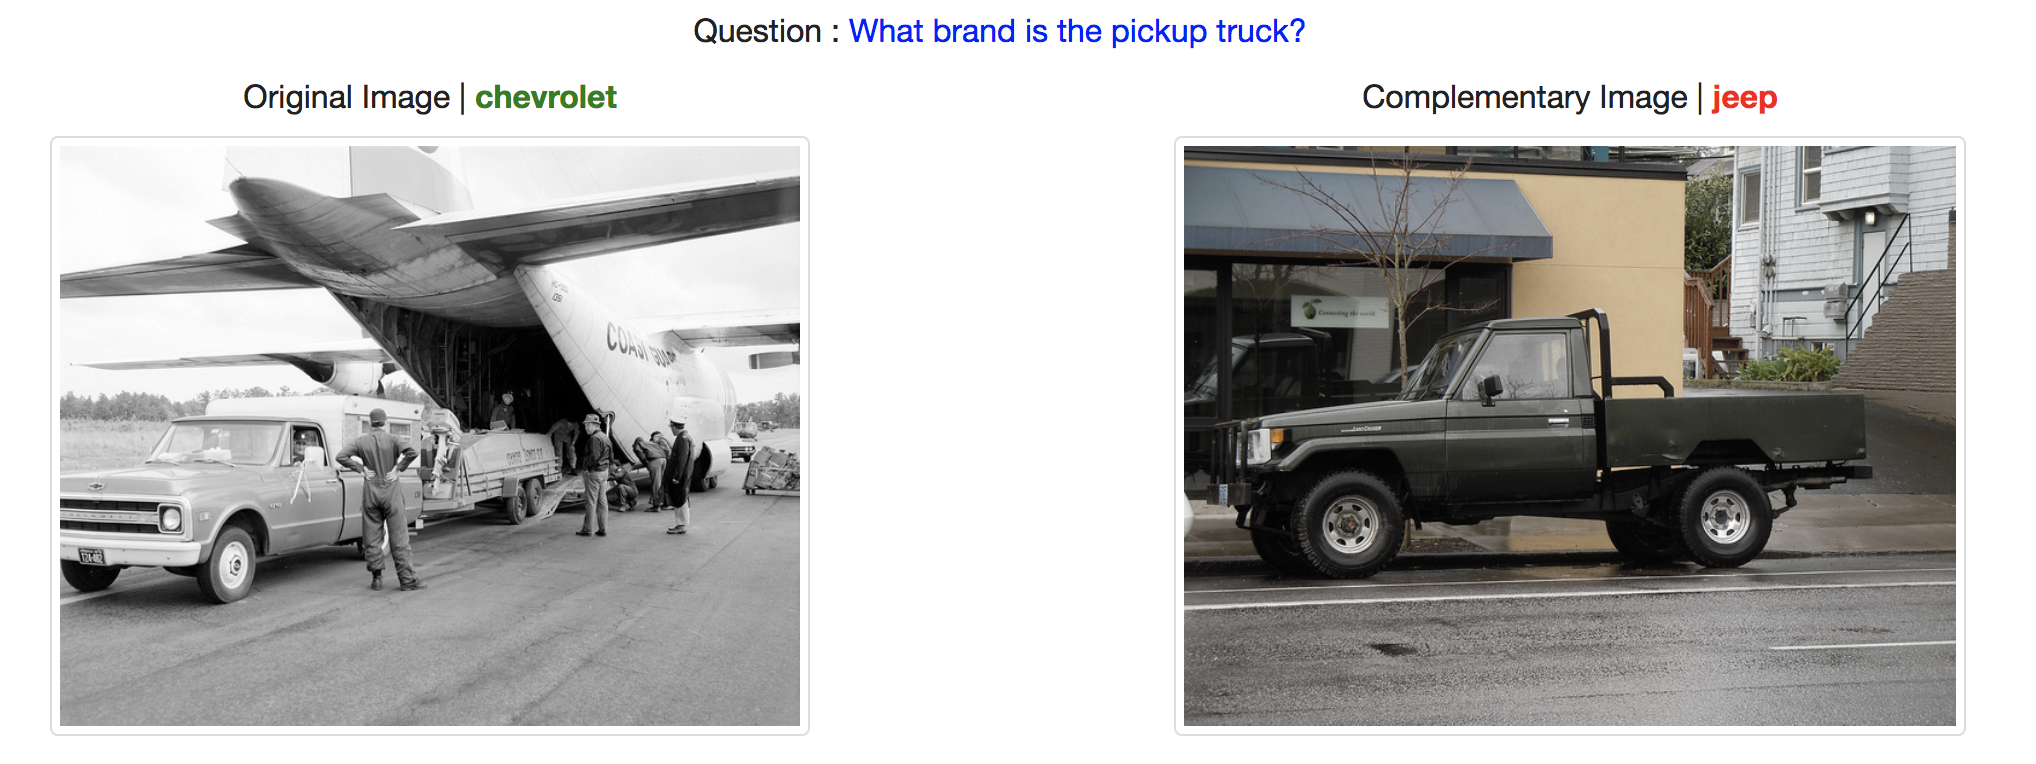
\includegraphics[width=0.8\textwidth]{vqa2-2.png}}
% 	\caption{VQA 2.0中针对同一问题的不同图像和答案实例}
% 	\label{vqa2}
% \end{figure}

\textbf{CLEVR}\qquad
为了更加准确地衡量视觉问答系统各个方面的推理能力,Johnson等人提出了一个结合语言和基本视觉推理诊断数据集CLEVR。CLEVR包含10万张由空间立方体组成的合成图像、将近100万个问题,其中包含85.3万个独特的问题。在图像的设置上,CLEVR为了减小识别难度,关注系统的视觉推理能力,采用了由空间立方体组成的合成图像,并且每张图像均有包含所有物体位置和属性的说明。CLEVR的问题也均由程序生成得到,涉及属性识别、计数、比较、逻辑运算等子任务。

% 为了减少问题的偏见,数据集生成的问题中有85\%是独特的;为了控制问题的准确性,数据集剔除了有歧义的问题,例如,询问“正方体右边的球体是什么颜色?”时,如果“正方体”右边有多个“球体”,问题便产生歧义,答案变得不唯一,使得评估过程变得复杂和不准确;为了保持问题的复杂性,数据集拒绝了一些看似复杂但实际上限定条件无效的问题,例如,询问“球体前面的圆柱体是否为金属的?”时,如果场景中仅有一个“圆柱体”,那么问题中的“球体前面”的限定便可以被忽略,这种情况降低了问题的复杂性。

% 由于CLEVR数据集对图像和问题具有完全的掌控,能实现其他数据集难以实现的能力测试,要求系统具有短期的记忆力、注意力机制、组合推理能力。
% 但同样因为其简单的图像场景设置,CLEVR不能测试出视觉问答系统在常识推理、复杂推理的表现,并且也不能衡量系统在真实场景中的识别能力和稳定性。
% \begin{figure}[H]
% 	\centering
% 	\subfigure[尺寸、形状、样色、材质的标注]{
% 		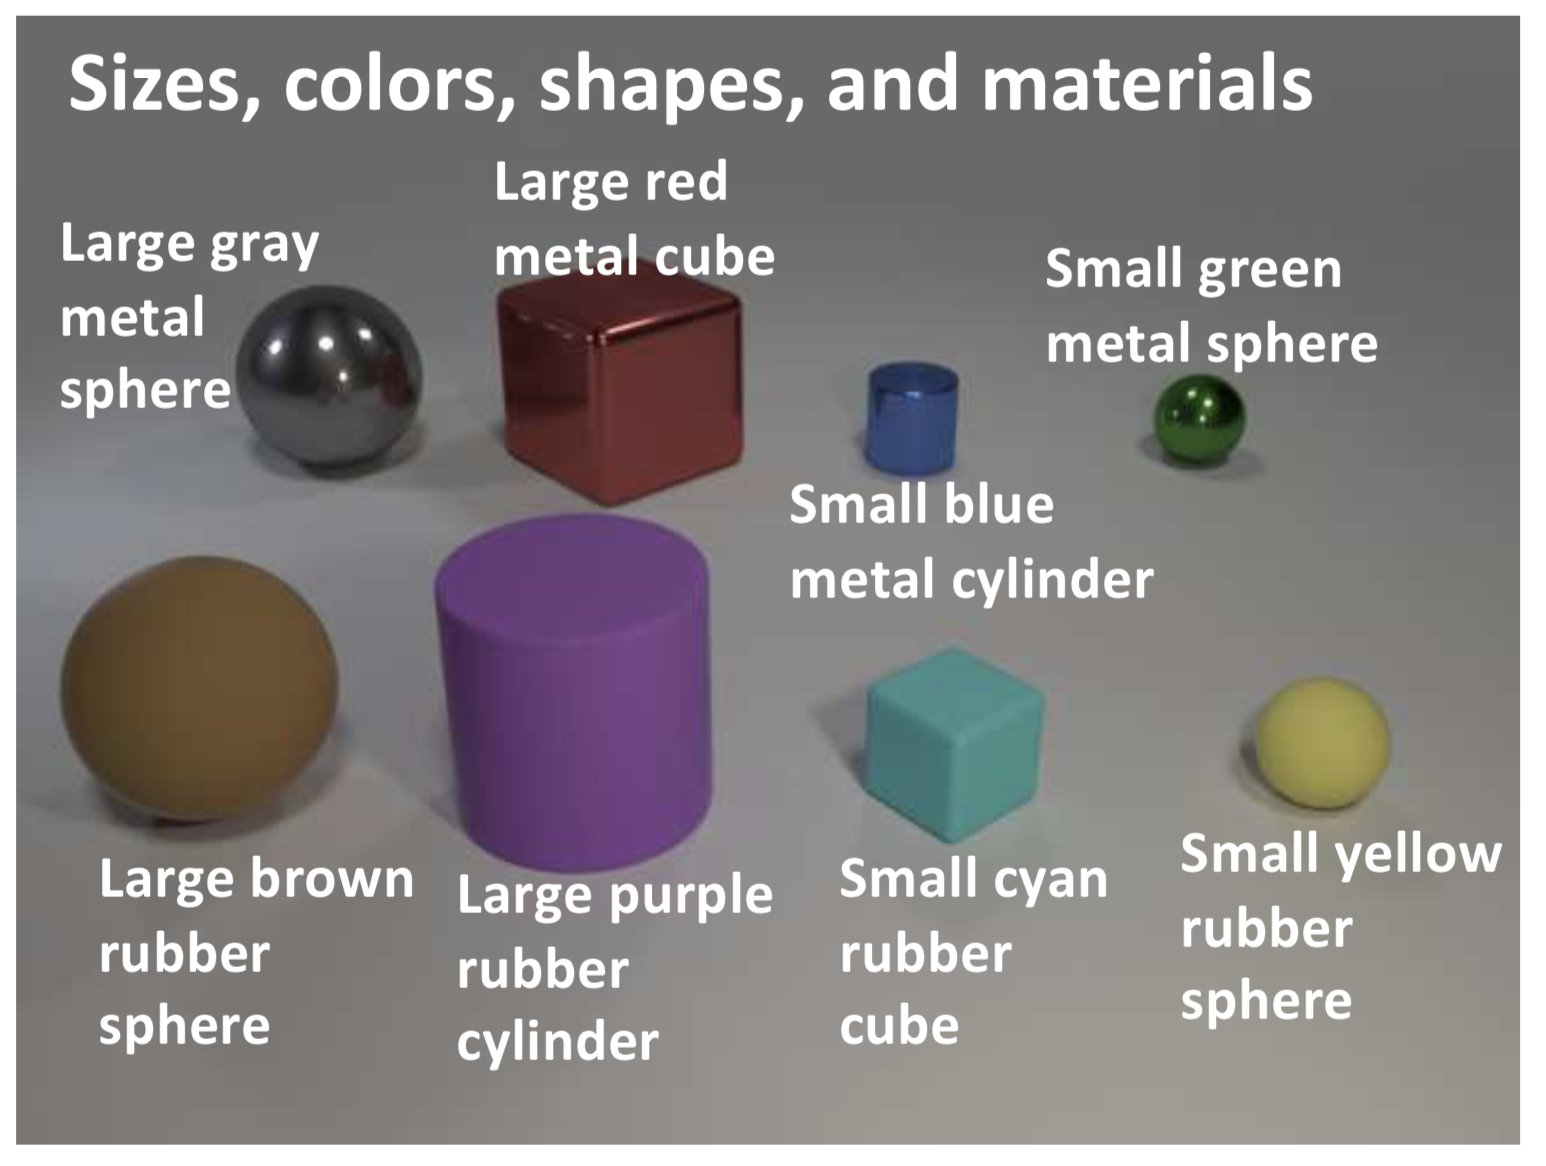
\includegraphics[width=0.3\textwidth]{clevr1.png}}
% 	\subfigure[空间左右的标注]{
% 		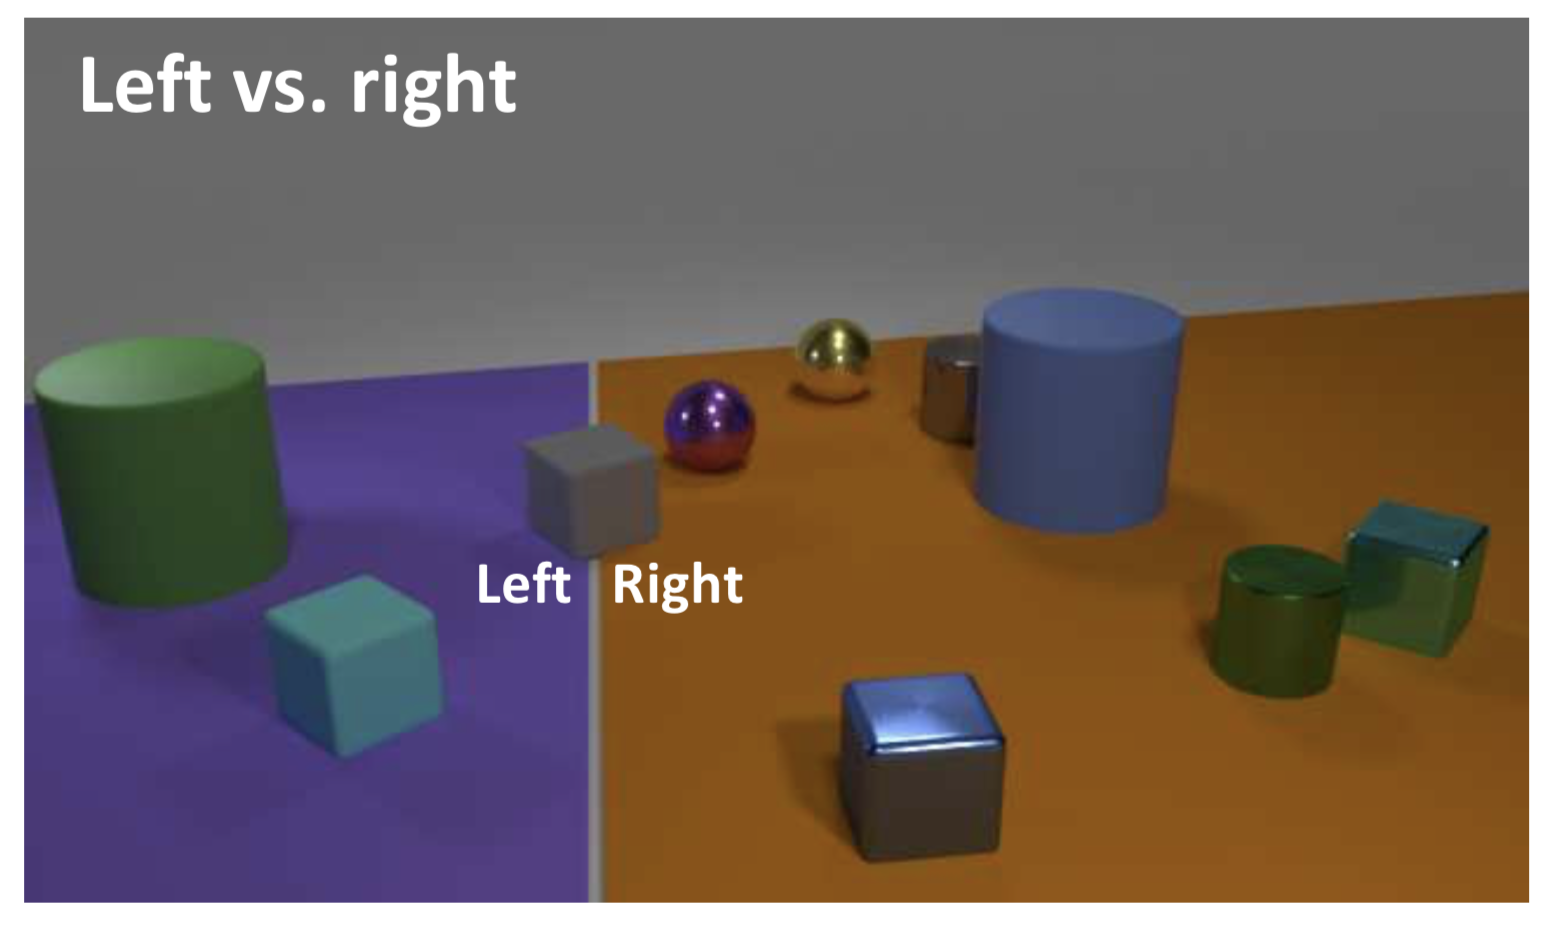
\includegraphics[width=0.3\textwidth]{clevr2.png}}
% 	\subfigure[空间前后的标注]{
% 		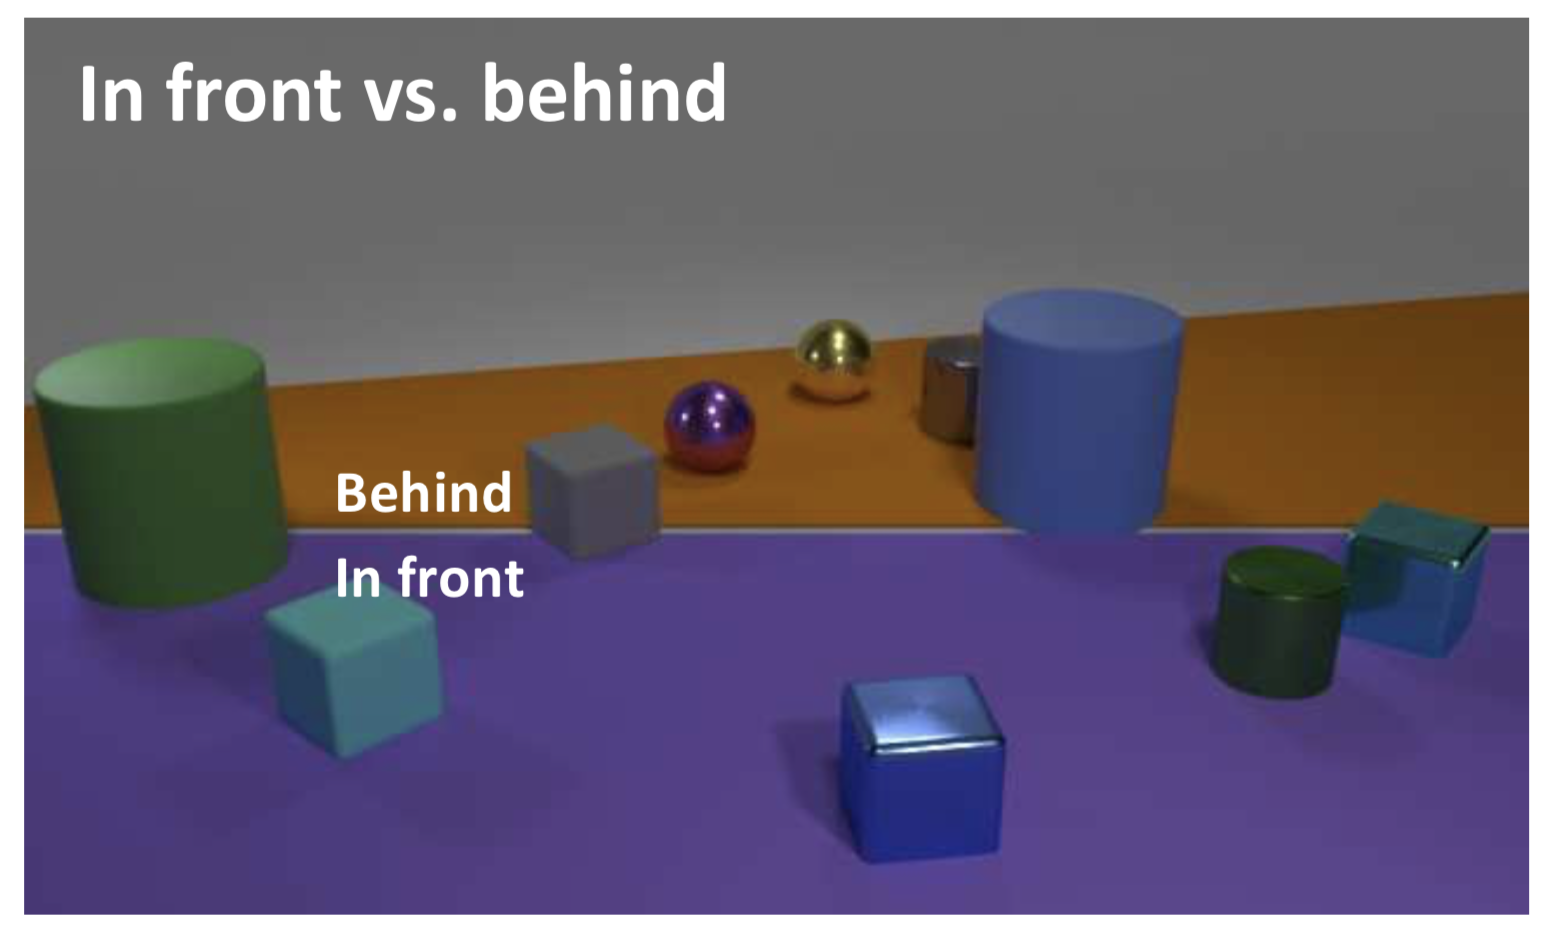
\includegraphics[width=0.3\textwidth]{clevr3.png}}
% 	\caption{CLEVR中图像标注}
% 	\label{clevr}
% \end{figure}

% \subsection{VQA-CP}
% 数据集一般会划分为训练集和测试集两个部分,在视觉问答任务中同样如此。如果训练集中的答案分布存在偏见,且测试集与训练集之间的答案分布相近,那么系统便可以通过记忆在训练过程中得到的数据偏见,并将其应用于测试过程,这样得到的准确率的可信度将会打折扣,例如,在训练集中询问颜色的问题中“白色”最为常见,同样在测试集中的“白色”也为热门答案,这回干扰系统的评估结果,不清楚系统是通过正确推理得到还是”经验“得到的。

% 针对训练集和测试集中问题答案分布相似的状况,VQA-CP重新对VQA数据集和VQA 2.0进行划分,重新划分得到的训练集和测试集在每个问题类型中的答案分布均不同,例如,在训练集中询问颜色的问题中,“白色”、“红色”为最常见的答案,而在测试集中“黑色”、“粉色”为最常见的答案;对于询问运动类型的问题,在训练集中“网球”为最多的答案,而在测试集中“滑雪”为最常见的答案(如图\ref{vqa-cp})。
% \begin{figure}[H]
% 	\centering
% 	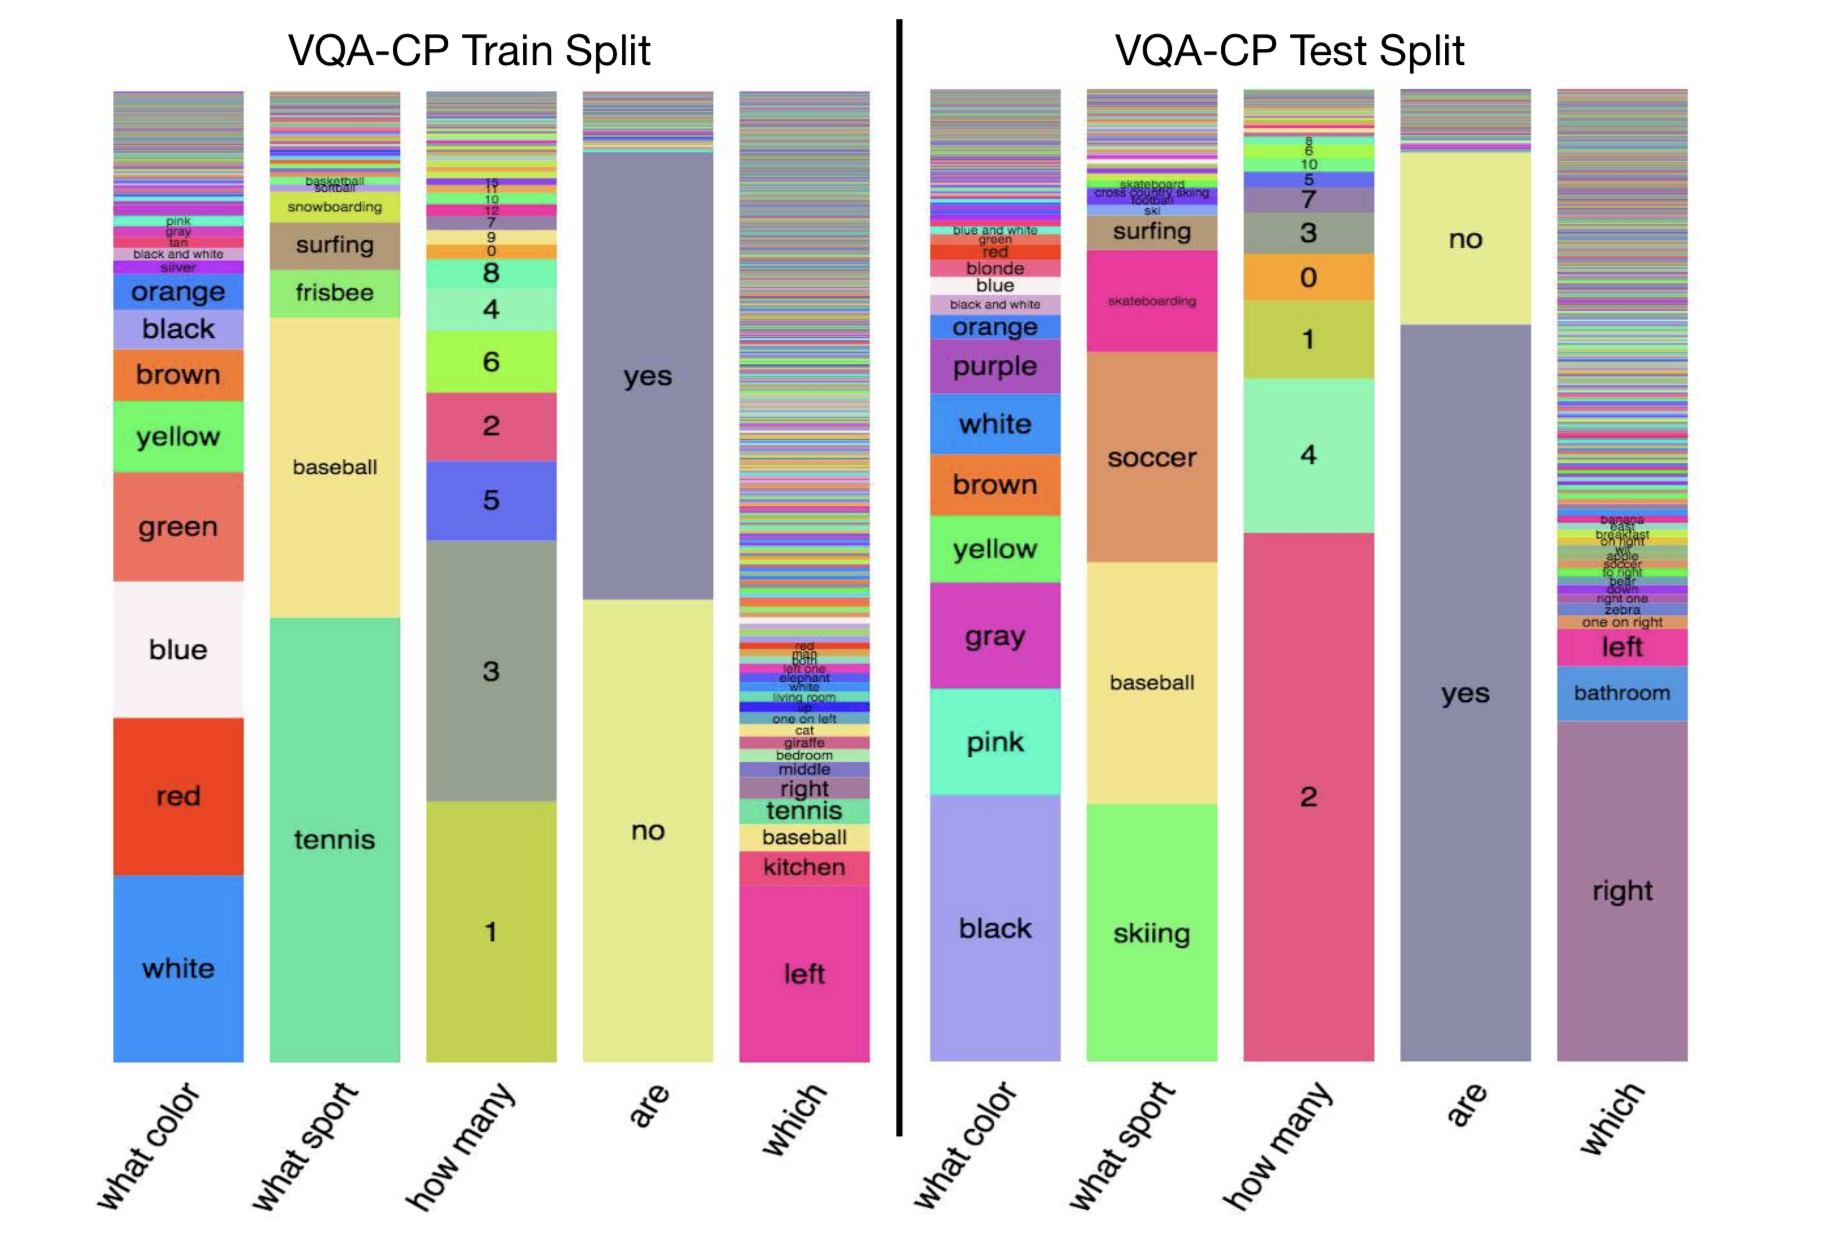
\includegraphics[width=5in]{vqa-cp.png}
% 	\caption{vqa-cp训练集和测试集的答案分布}
% 	\label{vqa-cp}
% \end{figure}

\subsubsection{基于知识的数据集}
\textbf{KB-VQA}\qquad
真实场景中的开放性问题可能涉及常识或者特定领域知识的先验知识,为了更好的评估VQA算法对需要高层次知识问题的准确推理能力,Wang等人构建了只包含复杂推理问题的数据集KB-VQA\citing{wang2015explicit}。

KB-VQA数据集从MS COCO\citing{lin2014microsoft}中挑选出700张图片样本,挑选出的图片包含150个物体类别和100个场景类别。每张图片附带有3-5个由人工生成的“问题-答案”对,所有的问题被限定在23种问题模板中,例如,“图片中是否存在某种概念?”,“图片中的某个物体被生产于什么地方?”等。
% ,详见\ref{qt}。

为了准确评估系统在需要先验知识的问题的表现,KB-VQA人工地赋予每个问题一个表示所需不同知识类型的标签,“视觉问题”、“常识问题”和“知识库问题”,其中“视觉问题”表示仅仅从图片中便可以获得答案的问题,例如,“物体是否存在于图片?”、“列出图片中包含的所有事物?”等,“常识问题”需要结合成人级别的常识和图像内容得出答案,例如,“图片涉及什么场景?”,“知识库问题”则需要某个领域特定的知识才能完成作答,例如,“图中的物品在哪一年被发明?”。数据集中的“视觉问题”、“常识问题”和“知识库问题”数量分别是1256、883和263。
% 23种问题模板在不同问题标签的分布如图\ref{qtd}。
% \begin{figure}[H]
% 	\centering
% 	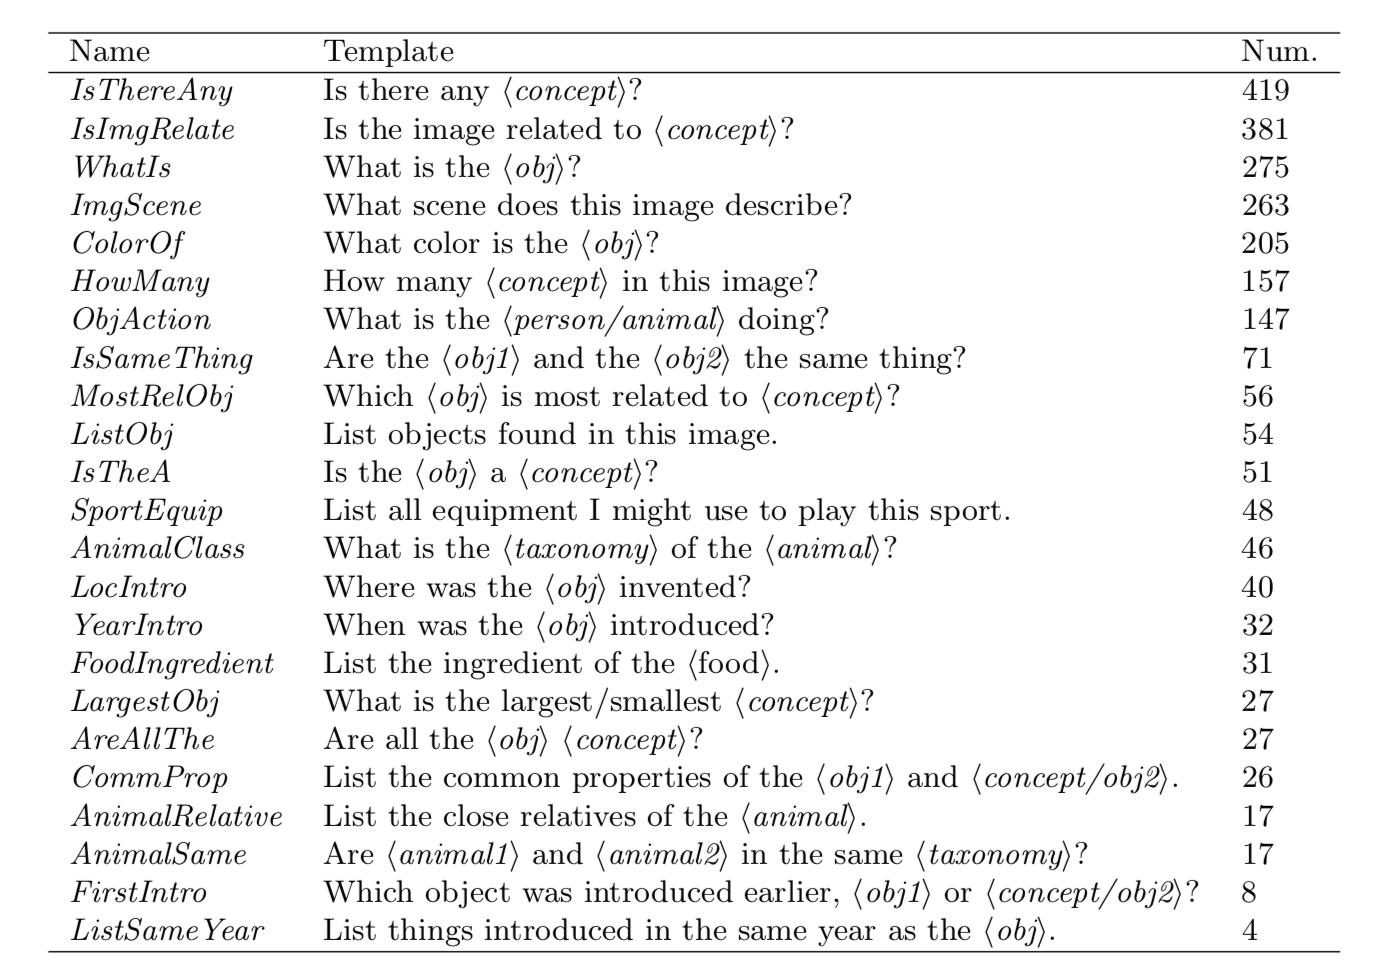
\includegraphics[width=0.8\textwidth]{qt.png}
% 	\caption{KB-VQA中23中问题模板及对应的问题数量}
% 	\label{qt}
% \end{figure}
% \begin{figure}[H]
% 	\centering
% 	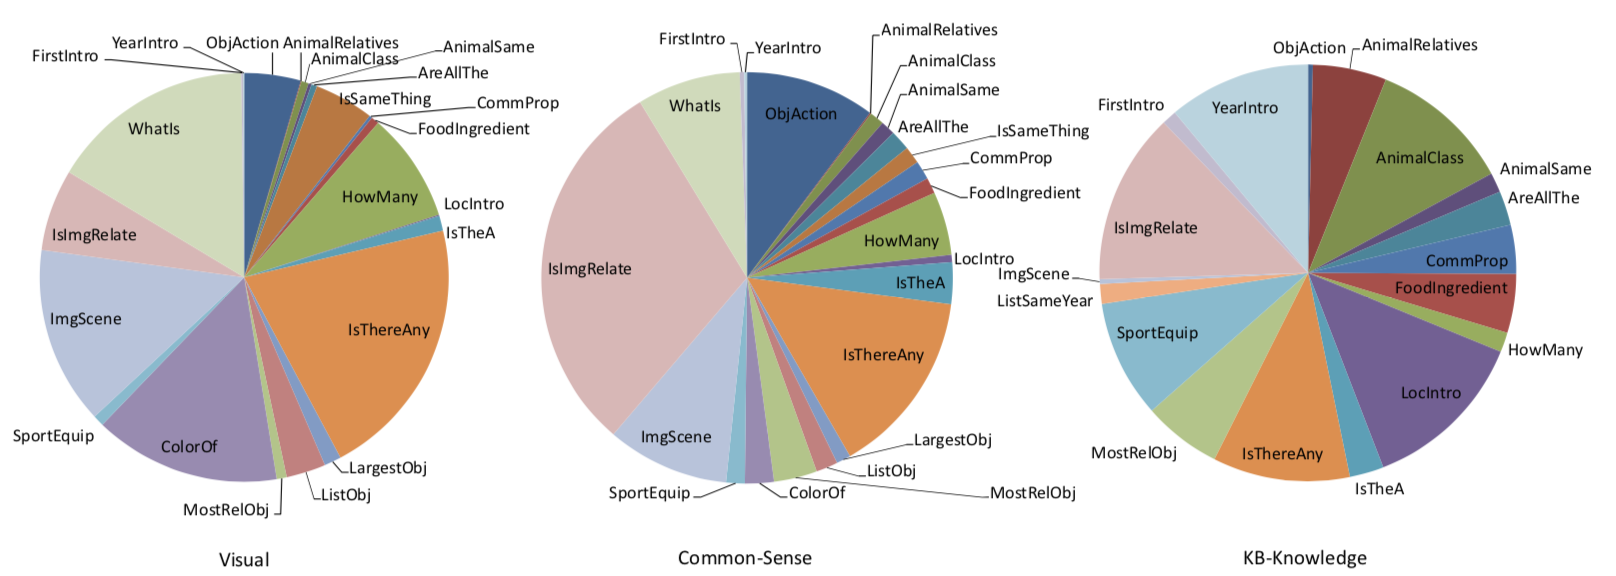
\includegraphics[width=0.8\textwidth]{qtd.png}
% 	\caption{KB-VQA中23中问题模板对应“视觉问题”、“常识问题”和“知识库问题”的分布情况}
% 	\label{qtd}
% \end{figure}

% 数据集中的“视觉问题”、“常识问题”和“知识库问题”数量分别是1256、883和263,就图片和问题的数量而言,KB-VQA数据集相较于COCO-QA等数据集是非常小的,而且从图\ref{qt}也容易看出,有16种问题类型的问题数量都不超过100个,甚至有个位数的问题数量,数据集的不均衡和小容量很难准确得评估出系统在细分问题类型上的推理能力。但需要先验知识的问题占比要远高于大型数据集,DAQUAR\citing{malinowski2014multi}几乎全是“视觉问题”,COCO-VQA\citing{ren2015exploring}仅仅包含5.5\%的问题需要常识,没有问题需要额外的知识库。

% KB-VQA在评估系统的复杂推理能力方面提供了一个解决方案,但数据集的容量、平衡性和多样性方面还需要更多的丰富,并且随着数据集的扩充,自动化和标准化的评估方式也相应的需要完善。

\textbf{FVQA}\qquad
为了评估视觉问答系统在需要先验知识的问题上的表现,Wang等人提出了FVQA数据集\citing{wang2017fvqa}。回答FVQA中的问题需要额外的知识,但不同于一般的数据集,FVQA将(图片,问题,答案)的三元组数据扩展为(图片,问题,答案,支持事实)的四元组形式,其中“支持事实”是回答问题所需要的额外知识,使用资源描述框架(RDF)的三元组形式,例如(猫,可以,爬树)。

FVQA从MS COCO\citing{lin2014microsoft}和ImageNet\citing{deng2009imagenet}中挑选出1906张图片,并对图片预处理,提取出三种类型的视觉概念:物体对象、场景和行为,最终提取出326种物体对象、21种场景和24种行为。为了获取与视觉概念相关的知识,FVQA以DBpedia\citing{auer2007dbpedia}、ConceptNet\citing{liu2004conceptnet}和WebChild\citing{tandon2014webchild}为知识源,从三种知识库中与视觉概念相关的所有知识中筛选出包含12种常见的谓语的知识,例如,关于分类的知识——“目录属于”、关于地点的知识——“地点所在”、关于大小比较的知识——“体积大于”。提取的知识以资源描述框架(RDF)的形式存储作为“支持事实”。数据集最终包含4608个需要先验知识的问题,涉及3458条事实。
% \begin{figure}[H]
% 	\centering
% 	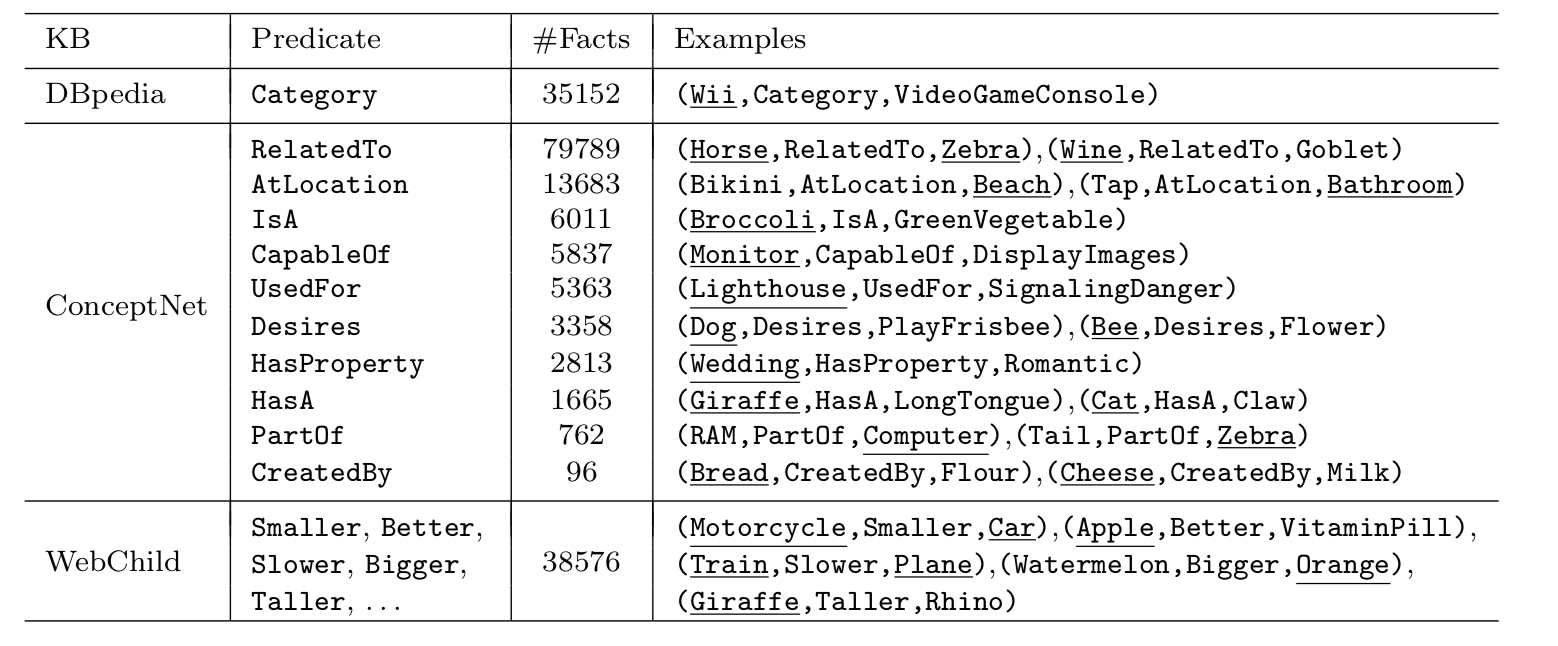
\includegraphics[width=0.8\textwidth]{fvqa_vc.png}
% 	\caption{从三种知识库中提取的知识涉及的12种谓语及相应的数量}
% 	\label{fvqa_vc}
% \end{figure}

% FVQA的问题和答案均使用人工的方式收集得到,被试者先选择图片中的一个视觉概念和一个与视觉概念相关的支持事实,再根据视觉概念和支持事实给出问题和答案,答案的来源要么是图片中的视觉概念要么是支持事实中涉及的概念。数据集最终包含4608个需要先验知识的问题,涉及3458条事实。根据视觉概念的类型,这些问题可以归为物体对象、场景和行为三种类型;根据支持事实的来源,可以归为DBpedia、ConceptNet和WebChild三种类型;根据答案来源,可以归为图片来源和知识库来源两种类型,不同分类在训练集和测试集的数量分布如图\ref{fvqa_cd}。
% \begin{figure}[H]
% 	\centering
% 	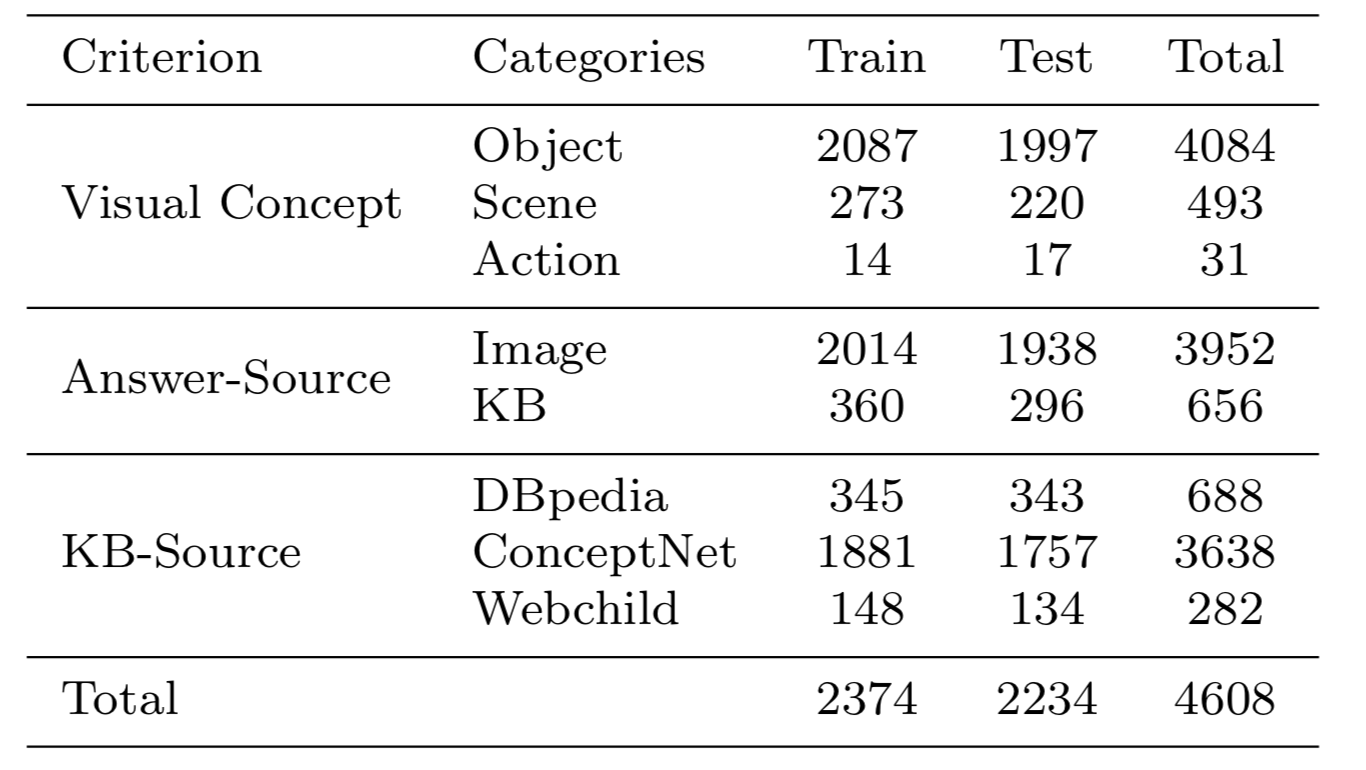
\includegraphics[width=0.8\textwidth]{fvqa_cd.png}
% 	\caption{不同分类在训练集和测试集的数量分布}
% 	\label{fvqa_cd}
% \end{figure}

% 从统计的数据上不难看出,绝大多数问题是针对图像中的物体对象,这与提供的视觉概念中物体对象的高占比有强关联,从知识来源上分析,答案除了能从图像中获得外,还包含14\%的答案需要从额外知识库中获得,并且问题中不包含“是或否”的二值问题,这降低了系统”猜中正确答案“的情况。

% FVQA和同样包含先验知识的数据集KB-VQA两者都能通过查询语言获取知识库中的数据,但不同于KB-VQA,FVQA拥更多的图片和问题数量,并且所有问题都需要额外知识。FVQA增加了ConceptNet和WebChild作为知识源,提高了知识库的多样性,能回答更多类型的问题,而不用预先设定问题模板。但FVQA数据集中几乎所有的答案都是物体对象,且为单个词语,不能训练模型给出对象关系的答案。FVQA数据集的支持事实多为单一谓语的句子,句式结构简单,如果用做训练集,不能考察模型应对多动词结构问题时的答案正确率。

% 然而两个数据集都面临着同样的问题:数据量的扩充和问题类型的扩充。两个数据集的问题收集都是通过人工的方式,并且参与者数量有限,因此直接导致了问题数量远低于其他自动化方法生成的数据集。大规模的协同工作和探索更多自动化方法是扩充数据集容量的方向。两个数据集都受到问题类型的限制,KB-VQA使用预先设定的问题模板,限制了问题的开放程度,FVQA虽然没有使用预先设定的问题模板,但其筛选的12种谓语间接的限制了问题的类型。

\section{视觉问答模型架构}
视觉问答任务要求系统能同时正确理解问题文本内容和图像内容,从视觉问答的处理过程可以看出,算法的核心有三个部分组成:如何提取出高层次的图像特征,例如,物体、属性、场景等;如何挖掘问题文本中的语义信息,以求能深入的理解问题内容,确定答案的形式和内容;如何结合图像特征和文本特征,得出正确或是最佳答案。

受神经网络在计算机视觉和自然语言处理成功应用的影响,从2014至今的视觉问答研究多采用了神经网络模型,并且模型基本上都由特征提取、注意力机制、特征融合、答案生成四个部分组成。模型使用卷积神经网络CNN提取图像特征,使用循环神经网络RNN或者长短期记忆LSTM处理文本信息,再通过不同的注意力机制增强特征的表达能力,最后融合特征,使用分类器输出答案,整体架构如图\ref{answer-generation}所示。
\begin{figure}[H]
	\centering
	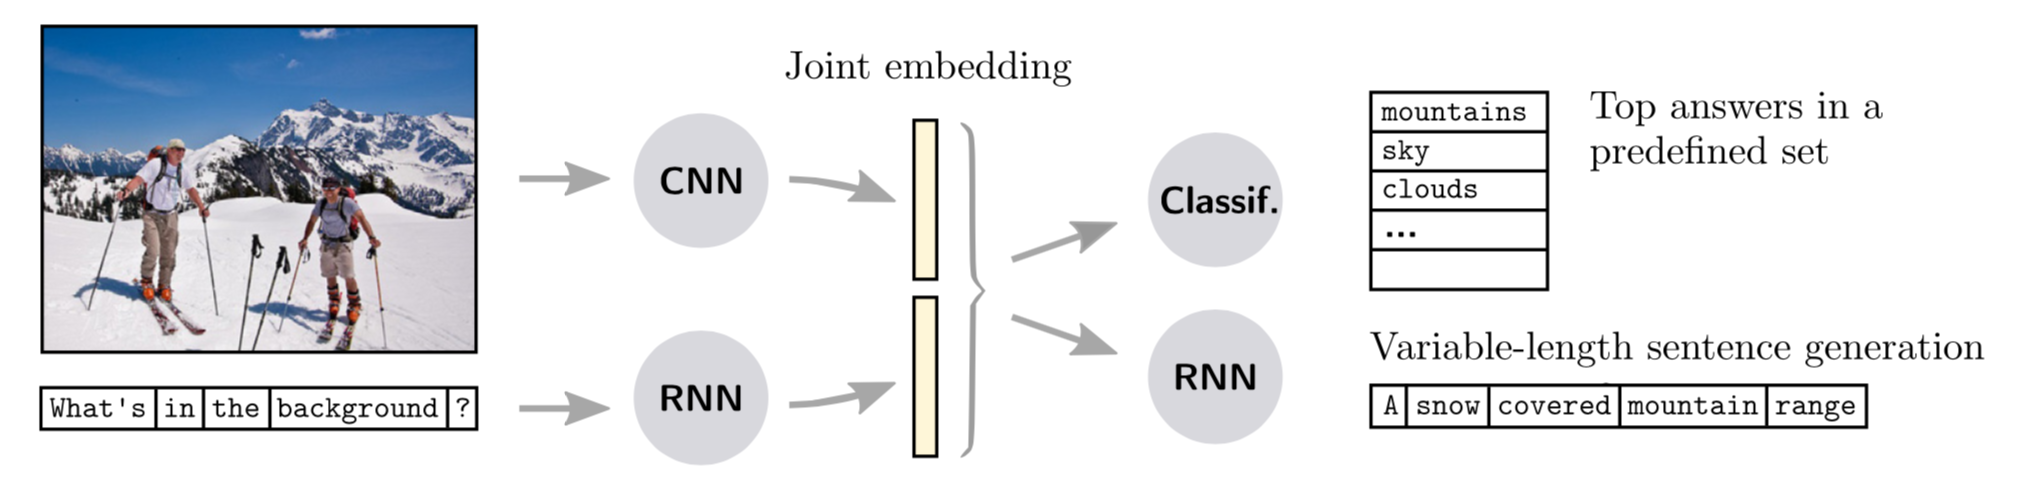
\includegraphics[width=0.8\textwidth]{answer-generation.png}
	\caption{VQA模型的一般架构}
	\label{answer-generation}
\end{figure}

% (1)特征提取部分一般由图像特征提取和文本特征提取两个部分组成,但一些引入知识库的模型中,可能会添加一个知识库特征提取部分,用于丰富特征。图像特征提取的方法一般使用预训练的卷积神经网络,例如VGGNet\citing{simonyan2014very}、 ResNet\citing{he2016deep}、GoogLeNet\citing{Szegedy_2015_CVPR}、Faster R-CNN\citing{ren2015faster}等。问题文本的特征提取则借鉴了自然语言处理中的成果,例如词袋模型(CBOW)\citing{zhou2015simple}、长短期记忆(LSTM)\citing{malinowski2015ask}、门控复发单位(GRU)\citing{noh2016image,kumar2016ask,xiong2016dynamic}。

% (2)注意力机制的引入也是跟随图像处理和自然语言处理的成功应用,通过对图像或文本特征不同部分分配有差异的权重值,从而更新特征,聚焦特征中重要的局部,实现特征增强。注意力机制能有效的抑制全局噪音,减少模型的无关运算,从而提高模型的准确性,在众多应用中均证明了其有效性。

% (3)特征融合是将提取得到的图像特征和文本特征映射到同一向量空间,并使用通过特征向量串联\citing{zhou2015simple}、卷积\citing{ma2016learning}、逐元素相乘\citing{antol2015vqa}、逐元素相加\citing{malinowski2015ask}等方法融合跨模态特征,便于后续的分类预测。对于视觉问答任务而言,图像特征和文本特征具有异质性,数据来源和特征分布都不同,因此好的特征融合对于模型的准确性具有重要的意义。

% (4)答案生成是解码融合后的特征,输出答案的部分。在视觉问答模型中,系统输出答案的方式有两种,最常见的方式是将任务视为分类问题,根据候选项的概率大小,确定答案。第二种方式则直接由系统合成答案语句,此类方法多出现在有额外知识库的视觉问答系统中,例如Attributes-LSTM\citing{wu2016value}、ACK\citing{wu2016ask}、Ahab\citing{wang2015explicit}、Facts-VQA\citing{wang2017fvqa}、Multimodal KB\citing{zhu2015building}。

\subsection{特征提取}
特征提取部分一般由图像特征提取和文本特征提取两个部分组成,但一些引入知识库的模型中,可能会添加一个知识库特征提取部分,用于丰富特征。图像特征提取的方法一般使用预训练的卷积神经网络。问题文本的特征提取则借鉴了自然语言处理中的成果,例如词袋模型(CBOW)\citing{zhou2015simple}、长短期记忆(LSTM)\citing{malinowski2015ask}、门控复发单位(GRU)\citing{noh2016image,kumar2016ask,xiong2016dynamic}。

\subsubsection{图像特征提取}
在卷积神经网络出现以前,图像的特征提取一般是使用人工设计特征,例如SIFT\citing{lowe1999object}、HOG\citing{dalal2005histograms}。虽然这些特征在特定任务上表现良好,但是其泛化性能较差,这意味着特征提取的成本较高。而卷积神经网络是一种深度学习模型,具有分层特征学习能力,以及更好的识别和泛化性能\citing{zeiler2014visualizing}。

卷积神经网络从机器视觉的成功应用开始,成为一众人工智能子领域的研究模型,已经被广泛用于物体检测、姿态检测、自然语言处理、语音识别等领域。并且随着迁移学习的兴起,大量性能优异的预训练卷积神经网络被用于图像特征提取,例如AlexNet\citing{krizhevsky2012imagenet}、VGGNet\citing{simonyan2014very}、 ResNet\citing{he2016deep}、GoogLeNet\citing{Szegedy_2015_CVPR}等。虽然有大量新的卷积神经网络被提出,但是它们都使用输入层、卷积层、池化层、全连接层和分类层组成的基本架构,如图\ref{cnn_structure}所示。
\begin{figure}[H]
	\centering
	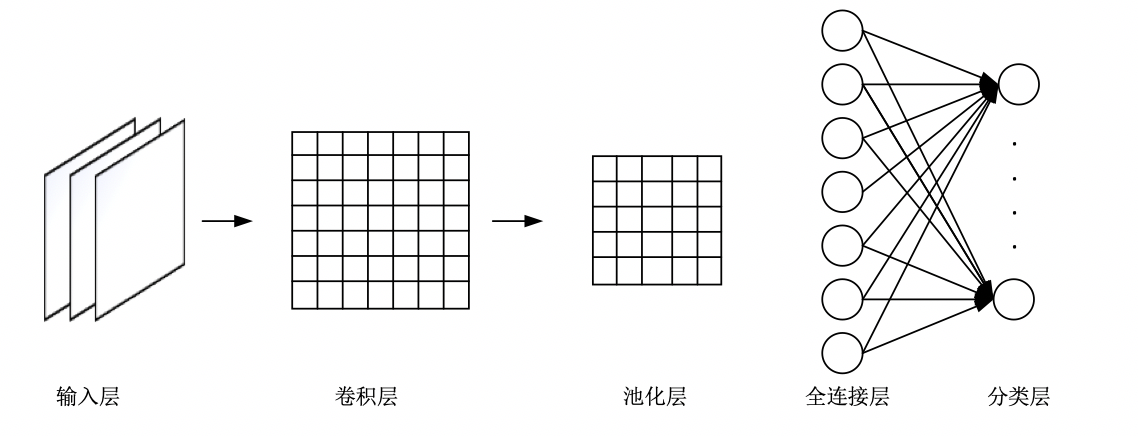
\includegraphics[width=0.8\textwidth]{cnn_structure.png}
	\caption{卷积神经网络的基本结构}
	\label{cnn_structure}
\end{figure}

卷积层是卷积神经网络的核心组成。对于高像素的彩色照片,全连接的神经网络将会产生大量参数,巨量的参数不利于模型的训练。卷积层的节点通过卷积核采样特征图的局部,并对局部的特征值进行卷积操作,再通过平移卷积核在特征图上滑动,从而扫描整张图片。不同的卷积核能够捕获图像的不同层次的特征,底层的卷积核得到的是边缘、颜色、纹理等粗粒度的特征,高层的卷积核则得到抽象的语义信息。给定输入图像I,$H_i$表示第i个卷积层的特征图,其中$H_0=I$,则相邻卷积层的特征图满足关系:
\begin{equation}
H_i = f(H_{i-1}\otimes W_i + b_i)
\end{equation}
其中,$W_i$表示第i层卷积核的权重向量,$b_i$表示第i层卷积核的偏置,$\otimes$表示卷积操作,$f$为非线性激活函数。常见的激活函数有Sigmoid, tanh, ReLu, Leaky ReLu, Maxout等,其中ReLu的公式为:
\begin{equation}
f(x) = max(0,x)
\end{equation}
因为其具有计算量小、收敛快等优点,被广泛用作激活函数。

池化层紧跟卷积层,对特征图进行下采样,降低特征维度,一方面能减少网络的计算复杂度,加快收敛,另一方面能提取主要特征。常见的池化方式有平均池化和最大值池化。

通过多个交替的卷积层和池化层后,特征进入全连接层和分类层,对每个类别进行概率预测,得到概率分布$Y$($l_i$表示第i个标签的类别)。因此整个卷积网络可以被视为接受输入$H_0$,在网络参数$W, b$的条件下,得到正确类别i的函数,如下式,
\begin{equation}
Y(i)=P(L=l_i | H_0; (W, b))
\end{equation}

网络的训练目标是最小化损失函数$L(W, b)$,从而更新模型参数。常见的损失函数均值平方、二值交叉熵、softmax交叉熵等。

\subsubsection{文本特征提取}
和众多自然语言处理任务一样,在视觉问答任务中如何准确理解问题内容对最终的答案准确率上有着决定性的影响。而自然语言理解中最为基本和核心的便是文本表达,文本表达将自然语言转换为计算机可处理的数字,为自动化处理文本相关的任务建立了基础。

在文本表达中,独热向量(one-hot)是最早也是最为简单的词向量。但是其稀疏性会带来的“维度灾难”和因简单的编码方式而造成“语义鸿沟”。基于分布式假设——即处于相似上下文的词语具有相似的含义,研究者先后提出了多种使用分布式表示的词向量模型,例如,CBOW,Skip-Gram,word2vec\citing{mikolov2013distributed},LSTM\citing{10.1162/neco.1997.9.8.1735}、潜在语义分析(LSA)\citing{landauer1998introduction},GloVe\citing{pennington2014glove}。

CBOW和Skip-Gram均是使用神经网络模型训练上下文信息得到词向量。word2vec也使用了CBOW与Skip-Gram来训练模型与得到词向量,但是并没有使用传统的DNN模型,而是使用霍夫曼树来代替隐藏层和输出层的神经元,提高了计算效率,因此被研究者广泛地使用作为预训练的词向量。但是由于word2vec使用滑动窗口来限定上下文信息,因此得到的词向量仅仅使用了局部的语义和语法信息。

循环神经网络(RNN)是处理序列化数据最为常用的模型,通过将句子中词特征循环迭代后,得到句子特征。但由于循环神经网络具有遗忘性,存在长时依赖问题,长短期记忆神经网络(LSTM)逐渐替代RNN。LSTM由三个门控制,分别是输入门、遗忘门和输出门。输入门控制着网络的输入,遗忘门控制着记忆单元,自动学习需要保存的记忆,输出门控制网络的输出。

不同于word2vec使用局部语料,潜在语义分析(LSA)采用统计计数的方式获得语料的全局信息,其统计预料库中每两个词共同出现的次数构成共现矩阵,并采用了基于奇异值分解(SVD)的矩阵分解技术对大矩阵进行降维,得到词向量。然而LSA方法中的SVD计算量很大,并且共现矩阵仅能表示两个词语同时出现的次数,并不能表示词语之间的远近关系。

为了改进word2vec的局部预料限制和LSA的计算复杂性,GloVe使用衰减函数改造LSA的共现矩阵,使得词语间的远近关系得以表达。GloVe还构建了词向量和共现矩阵之间的近似关系,使用梯度下降算法取代了LSA中的奇异值分解,大大减少了计算代价,并且得到了远超LSA和word2vec的性能。

以上提及的文本特征化方法被广泛的使用在视觉问答模型中。值得注意的是,以上方法都是将文本转换为固定的静态词向量,而静态词向量缺乏对上下文的感知,因此不能有效的表征多义词和具有多语法成分的词组。本文的重要改进之一便是引入动态词向量,具体内容将在N-KBSN模型架构中介绍。

\subsection{注意力机制}
人类获取外部视觉信息时,会自动形成一种“像素不均衡”,在同一视野范围内的像素被视觉中枢神经系统根据“关注区域”的远近、相关性特征自动分配不同的分辨率,使得“关注区域”内的像素具有极高的分辨率,而其他的像素仅仅作为视觉信息输入,并不参与大脑的语义处理(如图所示\ref{human-virtual})。因此视觉注意力机制帮助大脑过滤了低相关性的视觉信息,减少了待处理数据的体积,极大地提高了信息处理速率并松弛了大脑负载。
\begin{figure}[H]
	\centering
	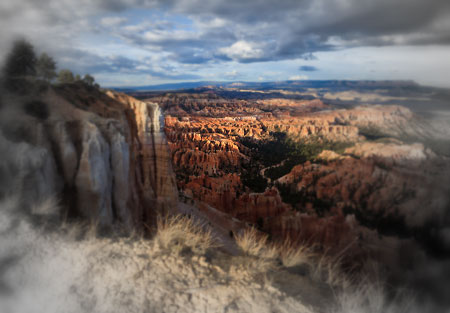
\includegraphics[width=0.5\textwidth]{human-virtual.png}
	\caption{人类视觉系统的“像素不均匀”现象}
	\label{human-virtual}
\end{figure}

近几年,受到人类视觉注意力机制的启发,在神经网络中引入注意力机制变得十分热门,在自然语言处理和计算机视觉领域的应用也极大得帮助了原有算法精度和计算效率的提升。Google Deepmind团队提出了一种带有注意力机制的循环神经网络(RNN),并成功应用于图像分类任务,获得了优于以往卷积神经网络(CNN)的基线水平的分类精度\citing{mnih2014recurrent}。随后,带有注意力机制的循环神经网络便被广泛应用于自然语言处理和计算机视觉的多个子领域\citing{bahdanau2014neural, xu2015show, NIPS2015_5847}。Bahdanau等人将注意力机制引入神经机器翻译任务,仍然使用“编码-解码”的翻译模式,但一改以往将源语言文本映射为一个固定长度的向量的编码方式,而是将原语言文本编码为向量序列,解码时将翻译和位置对应因素联合学习,训练向量序列中各向量对翻译词组的不同权重,加和完成翻译结果的推断,得到了以往最优的结果\citing{bahdanau2014neural}。Xu等人受到注意力机制在机器翻译和物体识别任务成功应用的启发,将带有注意力机制的循环神经网络应用于自动生成图像标注,并且在Flickr9k, Flickr30k 和MS COCO 三个数据集上均获得了最优的结果\citing{xu2015show}。随后,更多注意力机制的变型或优化研究均在图像标注任务上展开\citing{ 7243334, wu2017global, li2017image, lu2017knowing}。

相较起图像标注任务,视觉问答任务除了要求系统能理解图片内容,生成语义和句式合理的自然语言文本以外,还需要联合学习问题文本和聚焦与问题相关的图像细节。因此,在视觉问答模型中,从作用对象来分,注意力机制可以分为图像自注意力机制、文本自注意力机制、引导注意力机制。不同的模型使用的注意力机制细节不同,本文将使用多头注意力机制(Multi-head Attention, MA)实现图片的自注意力(V-SA)、问题文本的自注意力(Q-SA)、由问题引导的对图像的注意力(Guided Attention, GA),具体的实现细节详见N-KBSN模型。

\subsection{特征融合}
对于视觉问答任务而言,图像特征和文本特征具有异质性,数据来源和特征分布都不同,因此好的特征融合对于模型的准确性具有重要的意义。

多模态的融合方式可以分为协同表示和联合表示,协同表示是指将一种模态特征映射到另一种模态的特征空间,再融合;联合表示则是将不同模态的特征映射到同一特征空间。具体而言,协同表示是将图像特征映射到文本特征空间,再使用各类特种融合方法;联合表示则分别提取图像特征和文本特征,并且将两种特征统一维度,再进行相加或者拼接。联合表示的方式具有很高的灵活性,图像和文本特征的提取分开,并且融合的方式的选择也更为多样,因此目前大多模型均是使用该模式,本文也是使用联合表示,分别提取特征,再融合。

常用的特征融合方法有:向量串联\citing{zhou2015simple}、卷积\citing{ma2016learning}、逐元素相乘\citing{antol2015vqa}、逐元素相加\citing{malinowski2015ask},另有模型使用更复杂的特征融合方法,例如,动态参数层\citing{noh2016image}、多模态紧凑双线性池化方法(MCB)\citing{fukui2016multimodal}。

\subsection{答案生成}
答案生成是解码融合后的特征,输出答案的部分。在视觉问答模型中,系统输出答案的方式有两种,最常见的方式是将任务视为分类问题,根据候选项的概率大小,确定答案。第二种方式则直接由系统合成答案语句,此类方法多出现在有额外知识库的视觉问答系统中,例如Attributes-LSTM\citing{wu2016value}、ACK\citing{wu2016ask}、Ahab\citing{wang2015explicit}、Facts-VQA\citing{wang2017fvqa}、Multimodal KB\citing{zhu2015building}。

\section{本章小结}
本章从视觉问答任务的定义、问题类型和数据集三个方面介绍该领域的基本知识,其中,我们提出了一种按照答案与问题和图像相关性的问题分类标准。本章还介绍了视觉问答模型的一般架构,并从图像特征提取、文本特征提取、注意力机制、特征融合、答案生成五个方面展开说明了目前的实践情况以及原理和公式。
